\begin{table}[t]
    \centering
    \caption{\textbf{训练与推理效率。} 推理耗时指为 4430 个视频提取特征的时间。检索耗时是在 ActivityNet Captions 评测集上，对 15,753 条查询进行编码、计算相似度和排序的总时间。}
    \resizebox{\linewidth}{!}{
        \begin{tabular}{@{}lccccc@{}}
        \toprule
        \textbf{模型} &
        \makecell{\textbf{每轮训练} \\ \textbf{耗时（ms）}} &
        \makecell{\textbf{模型参数量} \\ \textbf{（百万）}} &
        \makecell{\textbf{推理耗时} \\ \textbf{（ms）}} &
        \makecell{\textbf{检索耗时} \\ \textbf{（ms）}} &
        \textbf{SumR} \\
        \midrule
        GMMFormer & 38079 & 12.85 & 5473 & 15016 & 146.0 \\
        HLFormer & 52866 & 28.43  & 6547 & 17001 & 154.9 \\
        GMMFormerV2 & 62458 & 30.79  & 6578 & 17263 & 154.9 \\
        \large \modelname{} & 52658 & 30.79  & 6556 & 17058 & 156.8 \\
        \bottomrule
        \end{tabular}
    }
    \label{tab:efficiency}
\end{table}
\begin{table*}[t]
\centering
 \caption{\modelname{} 的消融实验。最佳得分用\textbf{粗体}标出。}
\resizebox{\textwidth}{!}{
\begin{tabular}{cl ccccc c ccccc c  ccccc}
\toprule
\multirow{2}{*}{ID}&\multirow{2}{*}{\textbf{模型}}& \multicolumn{5}{c}{\textbf{ActivityNet Captions}} &  & \multicolumn{5}{c}{\textbf{Charades-STA}}&& \multicolumn{5}{c}{\textbf{TVR}} \\
\cmidrule{3-7} \cmidrule{9-13} \cmidrule{15-19}
&& \textbf{R@1} & \textbf{R@5} & \textbf{R@10} & \textbf{R@100} & \textbf{SumR} && \textbf{R@1} & \textbf{R@5} & \textbf{R@10} & \textbf{R@100} & \textbf{SumR} & & \textbf{R@1} & \textbf{R@5} & \textbf{R@10} & \textbf{R@100} & \textbf{SumR} \\
\midrule
\midrule
\rowcolor{ourscolor}
(0)& \textbf{{\large \modelname{}} （本文）}& \textbf{9.3} & \textbf{27.8} & \textbf{40.5} & \textbf{79.1} & \textbf{156.8} &&2.3 & \textbf{9.5} & \textbf{15.2} & \textbf{53.6} & \textbf{80.6} &&   \textbf{18.4} & \textbf{40.7} & \textbf{52.0} & \textbf{87.5} & \textbf{198.6}     \\
\midrule
\rowcolor{basegray}
\multicolumn{19}{l}{\scalebox{1.1}{\textit{多尺度视频间证据学习的有效性}}}\\
(1)& 仅帧尺度 & 8.6& 26.6 & 39.4 & 78.6 & 153.2&&2.4 & 8.8 & 14.6 & 52.6  & 78.4 &&  16.8& 38.4 & 50.5&87.5 & 193.1 \\
(2)& 仅片段尺度 & 8.5& 26.6 & 39.8 & 78.6 & 153.6&&2.4 & 8.6 & 14.4 & 52.6 & 78.0 &&  17.1& 38.8 & 50.6&87.6 & 194.1 \\
(3)& 移除聚合 & 8.7& 27.1 & 39.8 & 78.7 & 154.4&&2.3 & 9.2 & 14.9 & 52.6  & 79.1 &&  17.3& 40.2 & 51.5&87.7 & 196.7 \\
\midrule
\rowcolor{basegray}
\multicolumn{19}{l}{\scalebox{1.1}{\textit{划分融合策略的有效性}}}\\
(5) & 采信帧尺度 & 8.8 & 27.3 & 40.0 & 78.8 & 155.0 &&2.3 & 8.9 & 14.6 & 52.7 & 78.5 & & 17.2& 39.4& 50.6 & 87.5  & 194.7\\
(6) &采信片段尺度&  8.9 & 27.0 & 40.0 & 78.9 & 154.8  &&2.3 & 8.5 & 14.3 & 53.4  & 78.5 &&17.0 & 39.8 & 51.1 & 87.5  & 195.4\\ 
(7) &采用置信度主导&  9.1 & 27.4 & 40.1 & 78.9 & 155.5  &&2.3 & 9.3 & 14.8 & 53.0  & 79.3 &&17.9 & 40.0 & 51.4 & 87.8  & 197.0\\ 
\midrule
\rowcolor{basegray}
\multicolumn{19}{l}{\scalebox{1.1}{\textit{查询标签校准的有效性}}}\\
(8) & 移除校准 & 8.8 & 27.4 & 39.7 & 78.7 & 154.7 &&2.3 & 8.3 & 14.2 & 52.7 & 77.4 & & 17.4 & 39.7& 51.5 & 87.7  & 196.3\\
(9) & $\mathcal{\tilde{S}}_n$（仅校准该集合） &  9.1 & 27.6 & 40.1 & 78.9 & 155.6  &&2.3 & 9.0 & 15.0 & 53.1  & 79.4 &&17.7 & 40.4 & 51.4 & 87.8  & 197.3\\ 
\midrule
\rowcolor{basegray}
\multicolumn{19}{l}{\scalebox{1.1}{\textit{视频内证据学习的有效性}}}\\
(10) & 移除 $L_{\mathrm{intra}}$ 
& 8.7 & 27.1 & 39.7 & 78.6 & 154.0&&2.1 & 8.7 & 14.4 & 52.4 & 77.7 & & 17.3 & 39.2& 50.7 & 87.7  & 194.9\\
\midrule
\rowcolor{basegray}
\multicolumn{19}{l}{\scalebox{1.1}{\textit{灵活最优传输的有效性}}}\\
(11) & 采用 softmax & 8.7 & 27.3 & 40.0 & 78.7 & 154.7  &&2.3 & 8.6 & 14.2 & 53.5  & 78.6 & & 17.6 & 39.8& 51.2 & 87.5  & 196.1\\
(12) &采用 OT&  9.0 & 27.5 & 40.3 & 78.8 & 155.6  &&2.3 & 9.0 & 15.0 & 53.1  & 79.4 &&18.2 & 40.4 & 51.5 & 87.4  & 197.5\\ 
\hline
\bottomrule
\end{tabular}
}
 \label{tab:ablation}
\end{table*}
\section{实验} \label{sec:experiments}
\subsection{实验设置} \label{subsec:exp_setup}
\noindent \textbf{数据集} \quad 我们在三个基准数据集上进行实验。\textbf{(i)} ActivityNet Captions\cite{krishna2017dense} 约含 2 万个 YouTube 视频，平均时长为 118 秒，每个视频平均标注 3.7 个具有文本描述的时刻。\textbf{(ii)} Charades-STA\cite{gao2017tall} 包含 6,670 个视频和 16,128 条句子描述，平均每个视频包含 2.4 个时刻。\textbf{(iii)} TV Show Retrieval（TVR）\cite{lei2020tvr} 包含来自六部电视节目的约 2.18 万个视频片段，每个片段配有五条自然语言描述。为公平比较，采用与 MS-SL\cite{ms-sl} 相同的数据划分。

\noindent \textbf{评估指标} \quad 我们使用基于排名的指标 $R$@$K$（$K$ = 1, 5, 10, 100），即真实匹配项出现在前 $K$ 个结果中的查询百分比。另报告各召回率之和（SumR）以衡量总体性能。各项召回率以百分比（$\%$）表示。

\subsection{实现细节}
\noindent \textbf{数据预处理} \quad 对于 ActivityNet Captions 和 Charades-STA，分别采用\citet{zhang2020hierarchical} 和\citet{mun2020local} 提供的 I3D 特征作为视频表征。查询按 MS-SL\cite{ms-sl} 的做法编码为 1,024 维 RoBERTa 特征。对于 TVR，采用\citet{lei2020tvr} 发布的 3,072 维视频特征，由帧级 ResNet152\cite{he2016deep} 和片段级 I3D\cite{carreira2017quo} 表征拼接得到；相应文本编码为 768 维 RoBERTa 特征\cite{liu2019roberta}。

\noindent \textbf{实验配置} \quad 为保持模型规模一致，按照\cite{GMMFormerV2}，帧和片段编码器均采用 8 个高斯注意力块。潜在维度 $d = 384$。模型以 PyTorch 实现，并在单张 NVIDIA RTX 3080 Ti GPU 上训练 100 轮，其中第一阶段为 20 轮，批大小为 128。其他细节见附录 \ref{hyperparameter}。
\begin{figure}[t]
    \centering
        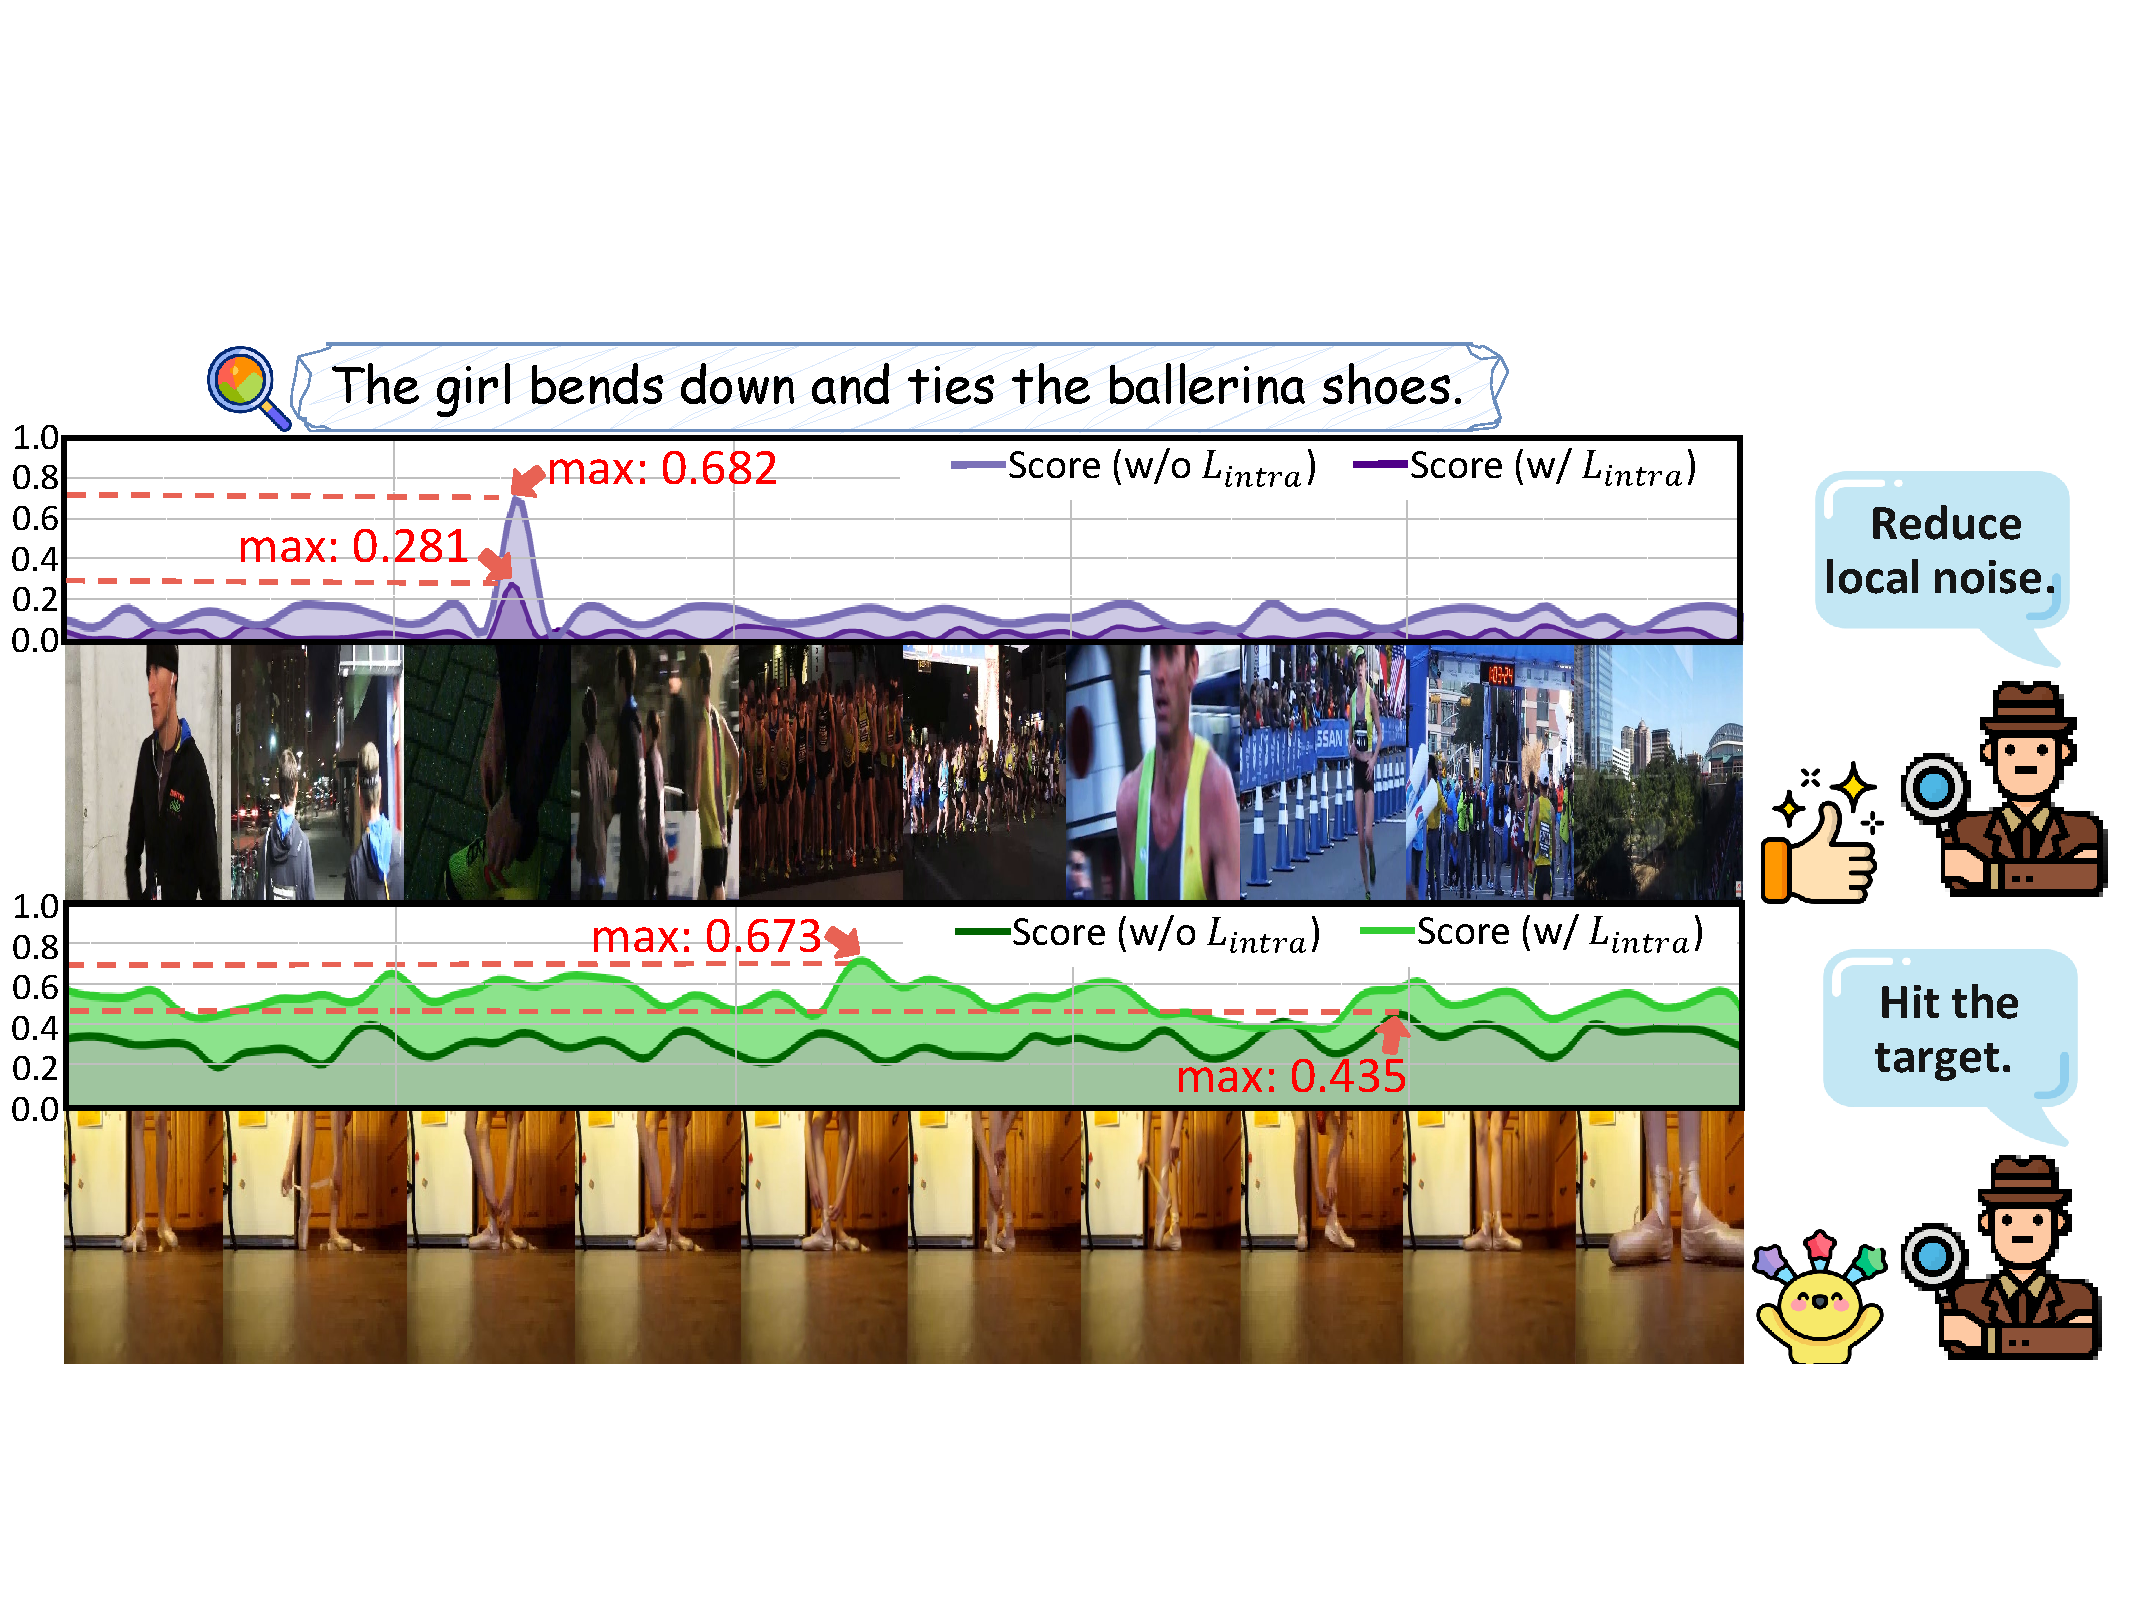
\includegraphics[width=\linewidth]{images/ablation_intra.pdf}
    \caption{使用\cref{fig:Intro} 中的同一组视频进行对比。移除 $L_{\mathrm{intra}}$ 后检索失败，无关视频得分高于真实匹配视频（0.682 对 0.435）。加入 $L_{\mathrm{intra}}$ 后，排序正确，真实匹配视频得分高于无关视频（无关视频为 0.281，真实匹配视频为 0.673）。}
    \label{fig:vis1}
    \vspace{-.3cm}
\end{figure}
\subsection{与先进方法对比}
\noindent \textbf{基线} \quad 我们选择 15 种有代表性的 PRVR 基线，并将 \modelname{} 与 T2VR 和 VCMR 方法进行比较。T2VR 对比方法包括 RIVRL\cite{dong2022reading}、CLIP4Clip\cite{luo2022clip4clip} 和 Cap4Video\cite{wu2023cap4video}。VCMR 对比方法包括 ReLoCLNet\cite{zhang2021video}、CONQUER\cite{hou2021conquer} 和 JSG\cite{jsg}。

\noindent \textbf{检索表现} \quad
\cref{tab:main} 汇总了各模型在三个基准上的检索表现。针对 PRVR 设计的方法整体优于 T2VR 和 VCMR 方法。\modelname{} 通过有效建模查询歧义、为更多视频片段提供可靠监督，达到了当前先进水平。具体而言，与最强竞争方法 DreamPRVR\cite{HLFormer} 相比，在 ActivityNet Captions 和 Charades-STA 上的 SumR 分别高 0.7 和 0.6。在 TVR 上，SumR 比 MGAKD\cite{MGAKD} 高 8.1。

\noindent \textbf{模型效率} \quad
\cref{tab:efficiency} 进一步比较了模型效率。所有结果为相同设置下 5 次运行的平均值。与规模相近的模型相比，\modelname{} 以相当的效率取得更好的性能，表明分层证据学习带来的开销很小。

\begin{figure}[t]
    \centering
    \parbox[b]{0.22\textwidth}{
        \centering
            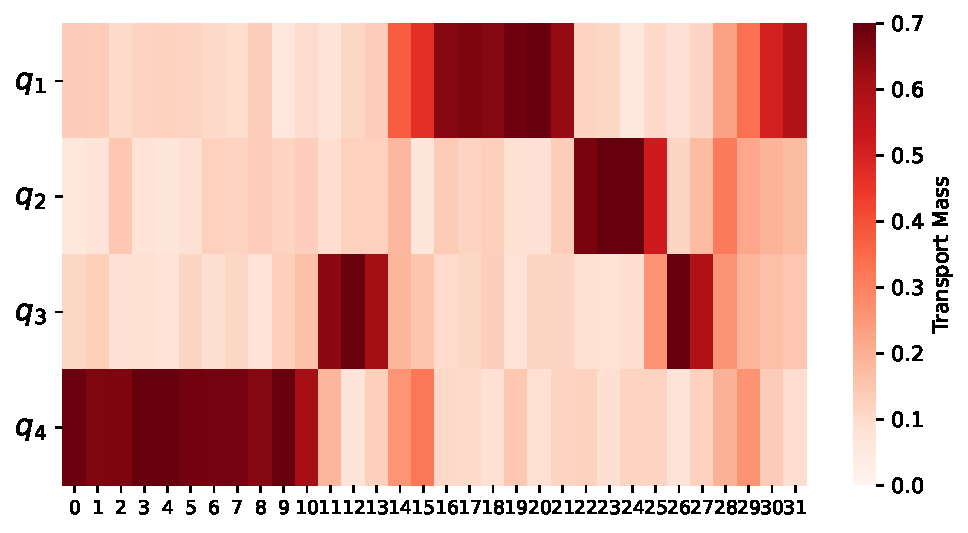
\includegraphics[width=\linewidth]{images/Standard_OT.pdf}
        \\[-0.45em]
        { \scalebox{0.85}{(a) 标准最优传输}}
    }
    \hspace{0.02\textwidth}
    \parbox[b]{0.22\textwidth}{
        \centering
            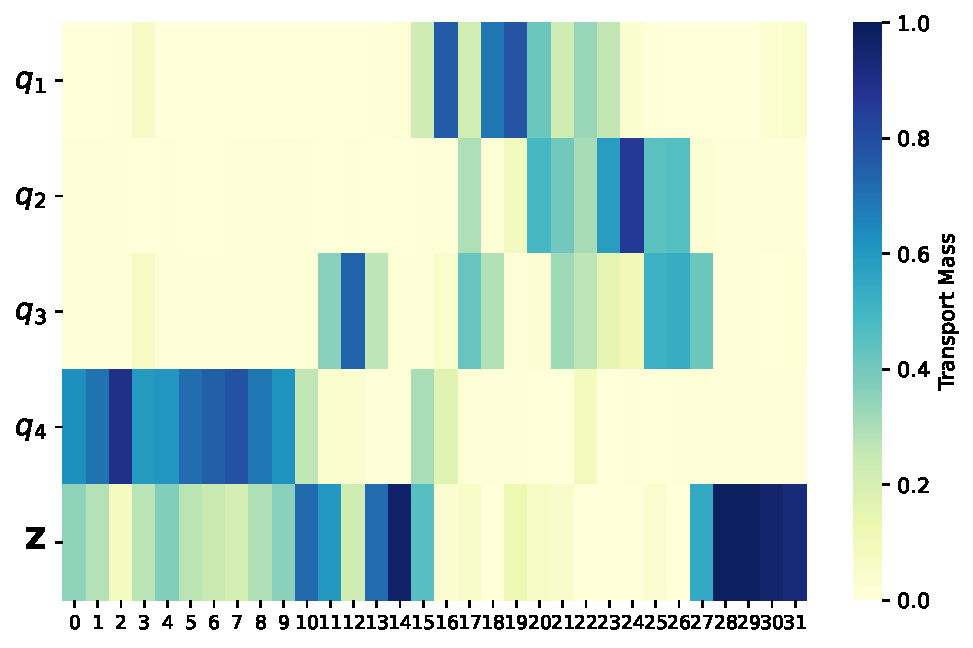
\includegraphics[width=\linewidth]{images/Flexible_OT.pdf}
        \\[-0.25em]
        {\scalebox{0.85}{(b) 灵活最优传输}}
    }
    \caption{OT 与 FOT 的传输质量对齐对比。$Z$ 表示回收槽。可视化结果显示，回收槽吸收了最后几个片段的传输质量。}
    \label{fig:pot}
\end{figure}
\subsection{模型分析}
\noindent \textbf{多尺度视频间证据学习} \quad
我们通过以下消融对多尺度分支进行评估：(i) 仅使用帧尺度或片段尺度分支，只用 $L^{f}_{U}$ 或 $L^{c}_{U}$ 训练；(ii) 移除动态协同证据聚合器，即训练时不使用 $L^{o}_{U}$。\cref{tab:ablation} 表明，单分支学习和移除聚合均会降低性能，说明多粒度视频间证据学习的必要性。结果还表明，跨分支证据聚合可提供整体不确定性估计，促进模型优化。

\noindent \textbf{划分融合策略的影响} \quad
我们比较三种策略：(i) 采信单一分支；(ii) 不确定性主导的划分融合（UDPF，默认），通过优先采信不确定性较高的类别处理分支冲突；(iii) 采用相反原则的置信度主导策略。\cref{tab:ablation} 表明，融合双分支预测可得到更可靠的划分并提高准确率。较为激进的置信度主导策略有时会产生过于自信却错误的关联，其性能低于较保守的 UDPF。

\noindent \textbf{查询标签校准的有效性} \quad
比较\cref{tab:ablation} 中编号 (0)、(8) 和 (9) 发现，未经校准的基线表现最差。我们认为，这是因为它忽略了固有的语义歧义，无差别地推远所有未配对视频，过度惩罚语义相关的样本，进而引入误导性监督。初步多义集合 $\tilde{\mathcal{S}}_n$ 又未能捕捉 $\tilde{\mathcal{S}}_p$ 中的多义查询，性能也非最优。这些结果进一步验证了对查询歧义建模和进行细粒度查询识别的重要性。


\noindent \textbf{视频内证据学习的有效性} \quad
\cref{tab:ablation} 中编号 (10) 的结果表明，移除 $L_{\mathrm{intra}}$ 会显著降低检索准确率。我们还在\cref{fig:vis1} 中可视化了查询与视频之间的时序注意力分数。加入 $L_{\mathrm{intra}}$ 后，模型降低了对无关视频的响应，减少了虚假局部尖峰，提高了相关视频的相似度分数。该目标通过一对多的软分配在查询和片段之间建立对应，汇聚多个相关片段的证据，从而提供更密集的时序监督，抑制虚假局部噪声，提高检索可靠性与准确率。


\noindent \textbf{灵活最优传输的作用} \quad
为了评估灵活最优传输的作用，我们比较三种变体：(i) 基于 softmax 的分配，(ii) 最优传输（OT），以及 (iii) 灵活最优传输（FOT，默认）。如\cref{tab:ablation} 所示，softmax 表现最差，OT 提升了性能，但无法捕捉 PRVR 中的部分相关性。如\cref{fig:pot} 所示，FOT 借助回收槽吸收噪声片段，减少由无关内容造成的错误对齐，因此表现最好。



\begin{figure}[t]
    \centering
        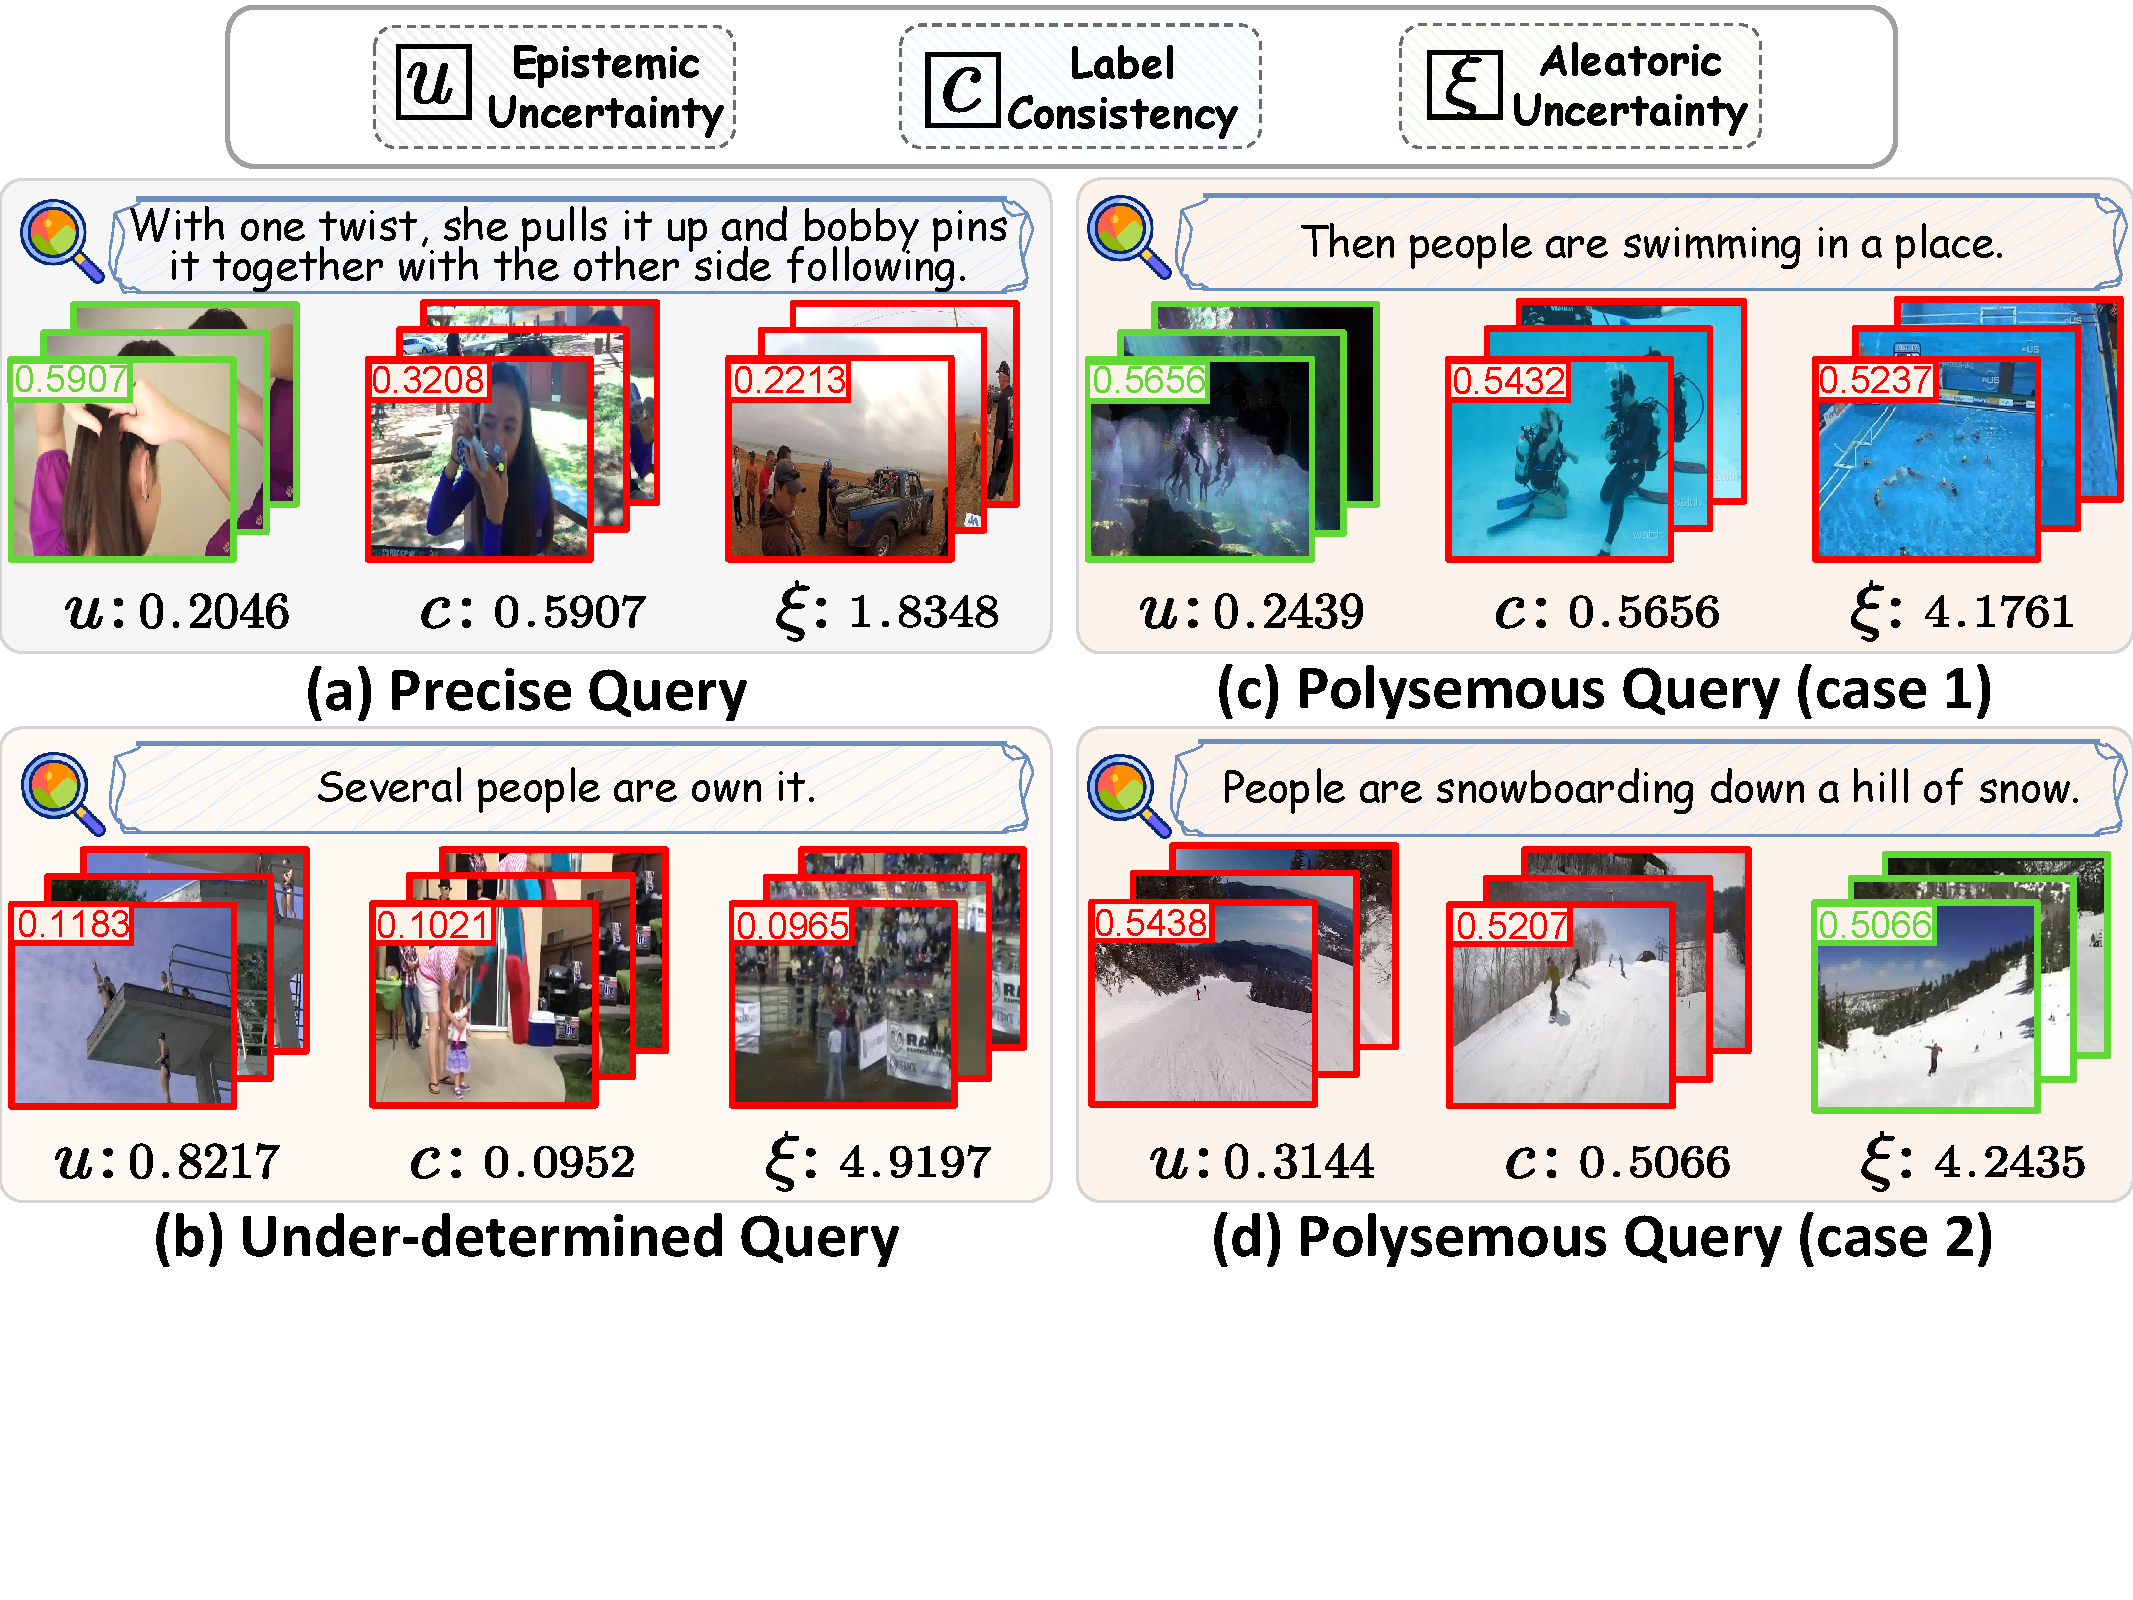
\includegraphics[width=0.48\textwidth]{images/query-choose.pdf}
    \caption{查询识别的定性示例。每条查询展示排名前三的视频，正确匹配用绿色边框标示，错误匹配用红色边框标示。每个视频的左上角显示相似度分数。}
    \label{fig:query-choose}
\end{figure}

\noindent \textbf{查询识别的定性结果} \quad
\cref{fig:query-choose} 展示了说明识别算法有效性的代表性示例。$u$ 与 $c$ 能清楚地分离信息不足查询，$\xi$ 则主要用于区分精确查询和多义查询，与我们的分类准则一致。我们观察到，相比缺乏明确指代线索且较短的多义查询，精确查询一般更长，也更具体。此外，信息不足查询可能含有语法或拼写错误（如误拼为 own），妨碍语义理解。这些观察符合实际场景，也进一步支持了本方法的有效性。
